
% Document class options:
% =======================
% blind: Anonymise all author, affiliation, correspondence
%        and funding information.
%
% lineno: Adds line numbers.
%
% serif: Sets the body font to be serif. 
%
% twocolumn: Sets the body text in two-column layout. 
% 
% num-refs: Uses numerical citation and references style 
%           (Vancouver-authoryear).
%
% alpha-refs: Uses author-year citation and references style
%             (rss).
%
% Using other bibliography styles:
% =======================
%
% To specify a different bibiography style
%
% 1) Do not use either num-refs or alpha-refs in documentclass.
% 2) Load natbib package with the options set as needed.
% 3) Use the \bibliographystyle command to specify the style
% 
% Included NJD styles are: 
%   WileyNJD-ACS
%   WileyNJD-AMA
%   WileyNJD-AMS
%   WileyNJD-APA
%   WileyNJD-Harvard
%   WileyNJD-VANCOUVER
%
% or you may upload an alternative .bst file 
% (if requested by the journal).
%
% Examples:
% =======================
%% Example: Using numerical, sort-by-authors citations.
\documentclass[twocolumn, serif, meta, authordate]{jote-article}


\addbibresource{nelson.bib}



%% Example: Using author-year citations and anonymising submission
% \documentclass[blind,alpha-refs]{wiley-article}

%% Example: Using unsrtnat for numerical, in-sequence citations
% \documentclass{wiley-article}
% \usepackage[numbers]{natbib}
% \bibliographystyle{unsrtnat}

%% Example: Using WileyNJD-AMA reference style and superscript
%%          citations, two-column and serif fonts for AIChE
% \documentclass[serif,twocolumn,lineno]{wiley-article}
% \usepackage[super]{natbib}
% \bibliographystyle{WileyNJD-AMA}
% \makeatletter
% \renewcommand{\@biblabel}[1]{#1.}
% \makeatother

% Add additional packages here if required
\usepackage{siunitx}


\usepackage{float}
\usepackage{bookmark}
\usepackage{lipsum}
% Update article type if known
% Include section in journal if known, otherwise delete
\papertype{META-RESEARCH}

\title{Towards an Expanded Understanding of Publication Bias}

% List abbreviations here, if any. Please note that it is preferred that abbreviations be defined at the first instance they appear in the text, rather than creating an abbreviations list.
%\abbrevs{ABC, a black cat; DEF, doesn't ever fret; GHI, goes home immediately.}

% Include full author names and degrees, when required by the journal.
% Use the \authfn to add symbols for additional footnotes and present addresses, if any. Usually start with 1 for notes about author contributions; then continuing with 2 etc if any author has a different present address.
\author[1]{Nicole Nelson}
\authorone{Nicole Nelson}


%\contrib[\authfn{1}]{Equally contributing authors.}

% Include full affiliation details for all authors
\affil[1]{Department of Medical History and Bioethics at the University of Wisconsin–Madison. Other affiliations are with the Holtz Center for Science and Technology Studies and the History department}
%\affil[2]{Department, Institution, City, State or Province, Postal Code, Country}


\corremail{\href{mailto:nicole.nelson@wisc.edu}{nicole.nelson@wisc.edu}}

%\presentadd[\authfn{2}]{Department, Institution, City, State or Province, Postal Code, Country}

\paperdoi{10.36850/mr2}

% Include the name of the author that should appear in the running header
\runningauthor{Nelson}

\jname{Journal of Trial and Error}
\jyear{2020}
\jissue{1}
\jvolume{1}
\jwebsite{https://www.jtrialerror.com}
\paperreceived{18 July, 2020}
%\paperrevised{7 September, 2020}
\paperaccepted{7 September, 2020}
\paperpublished{26 October, 2020}
\paperpublisheddate{2020-10-26}



\jpages{52-58}
\jlogo{media/jote_logo_full.png}


\abstracttext{\noindent This short essay argues for an expanded conception of publication bias. In addition to considering the selective publication of results, I argue that we need to also consider the selective publication of epistemic by-products—observations and knowledge that scientists accumulate incidentally in the process of carrying out their work. There are three reasons why we should be concerned about the exclusion of epistemic by-products from the published literature: first, because they play an important role in robust replication attempts; second, because their absence can result in misplaced scientific certainty; and third, because they contribute to a holistic understanding of natural phenomena. However, identifying and addressing publication bias against epistemic by-products and other undervalued forms of knowledge is more difficult than identifying bias against quantitative findings. I argue that scientific pluralism and making data publicly accessible are two potential remedies for addressing this form of publication bias. }

%\rolling{YES}

\heightabstract{45mm}
\widthaffil{40mm}

\setlength{\parskip}{0pt}


\keywordsabstract{epistemic by-products, publication bias, replication geneticization, scientific pluralism}

\begin{document}
%\cleartoleftpage
\setcounter{page}{52}
\pdfbookmark[0]{Nelson, N.  - Towards an Expanded Understanding of Publication Bias}{nelsonpdf}
\begin{frontmatter}
\maketitle

\begin{abstract}
%\phantomsection
%\addcontentsline{toc}{section}{Abstract}

This short essay argues for an expanded conception of publication bias. In addition to considering the selective publication of results, I argue that we need to also consider the selective publication of epistemic by-products—observations and knowledge that scientists accumulate incidentally in the process of carrying out their work. There are three reasons why we should be concerned about the exclusion of epistemic by-products from the published literature: first, because they play an important role in robust replication attempts; second, because their absence can result in misplaced scientific certainty; and third, because they contribute to a holistic understanding of natural phenomena. However, identifying and addressing publication bias against epistemic by-products and other undervalued forms of knowledge is more difficult than identifying bias against quantitative findings. I argue that scientific pluralism and making data publicly accessible are two potential remedies for addressing this form of publication bias. 
% Please include a maximum of seven keywords
\end{abstract}
\end{frontmatter}

\phantomsection \addcontentsline{toc}{section}{Introduction} \section*{Introduction}
Publication bias (also known as selective publication, or the "file drawer'' problem) has long been recognized as a problem in the sciences \parencite{Dickersin1990, Dickersin1987, Rosenthal1979}. The term describes problems arising from how scientists choose which studies (or which elements of studies) to publish from the many studies that they have conducted. If researchers decide whether to publish based on a property of the result—say, whether the result reaches commonly-used thresholds of statistical significance or supports the researcher's hypothesis—then the subset of study results that appears in the published literature will be biased.

In this short essay, I argue for an expanded conception of publication bias. In addition to considering the selective publication of results, I argue that we need to also consider the selective publication of \emph{epistemic by-products}—observations and knowledge that scientists accumulate in the process of carrying out their work \parencite{Nelson2018}. Researchers typically choose not to publish these findings not because they fail to reach statistical significance, but because they were never intended to be knowledge in the first place. This implicit distinction between the entities that scientists consider to be scientific findings and those that they consider to be anecdata, tacit knowledge, or lab lore acts as an additional filter that prevents some types of knowledge from circulating widely. Expanding the notion of publication bias to include these processes allows for a deeper understanding of how users of the scientific literature might arrive at a false sense of certainty, and also offers insight into how gaps form between individuals' understanding of natural phenomena.

\phantomsection \addcontentsline{toc}{section}{Existing research on publication bias} \section*{Existing research on publication bias}

Researchers studying publication bias have tended to focus on studies that have clearly specified questions, and outcomes that are assessed with quantitative measurements. Studies that ask questions such as ``Is psychotherapy effective?'' or ``Does smoking increase risk of heart disease?'' can be grouped in a way that allows researchers to define a universe of studies and then ask questions about the subset of those studies that appear in the published literature. The quantitative measurements typically employed in these studies---\emph{p}-values, effect sizes, hazard or odds ratios, correlation coefficients, and so on---allow researchers to compare across studies to look for evidence of bias. For example, ``funnel plots'' of outcome measures allow researchers to visually detect bias in the group of studies that they have collected \parencite{Begg1994, Egger1997}. In these plots, the effect sizes of the individual studies should theoretically be evenly distributed across the plot, and a plot where studies are clustered to one side allows researchers to see a ``missing mass'' of unpublished studies (Figure \ref{fig:figure1}). Multiple proposals for new techniques to visualize and quantify publication bias have emerged in the past few years \parencite{Schimmack2020, Simonsohn2013, vanAssen2015}.

\begin{figure}[h]
\centering 
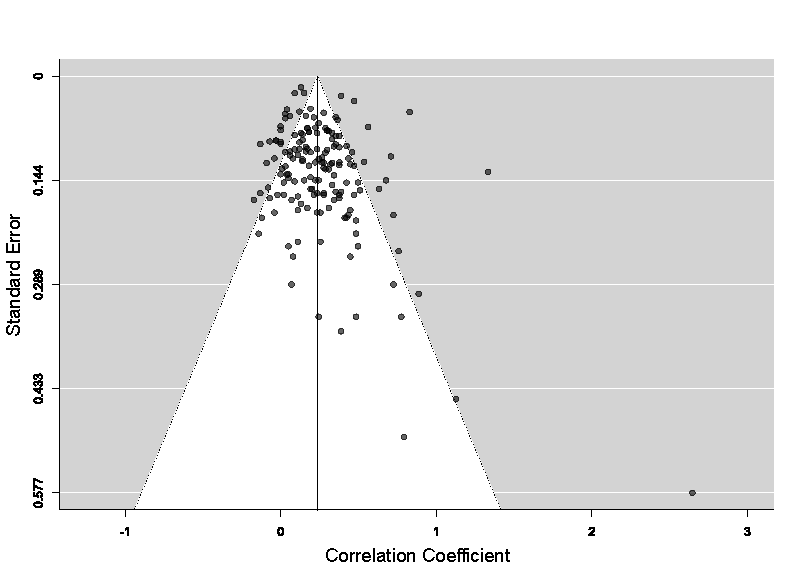
\includegraphics[width=\columnwidth]{media/betternelson.pdf}
\caption{\textbf{Sample funnel plot of a data set suggesting publication bias}. Plot of published studies examining the correlation between predictions of job performance made during interviews and actual job performance. Each point represents one study, where the \emph{x}-axis represents the correlation coefficient found in that study, and the \emph{y}-axis represents the precision of the study (measured by standard error). The white triangle indicates the 95\% confidence interval for the data set (that is, the zone where 95\% of the points should lie, assuming a normal distribution, homogeneity of variance, and no publication bias). The asymmetry in the plot indicates a ``missing mass'' of studies on the left side, suggesting that some studies that found no correlation or negative correlations were not published. The data underlying this plot is publicly available in the R package ``metafor,'' and an in-depth discussion of publication bias using this data set as an example is available in \parencite{Rothstein2005}.}
\label{fig:figure1}
\end{figure}



The main harms of publication bias, according to this research, are that evidence will appear more certain or interventions will appear more effective than they actually are. If the studies that find weak effects or no effects for an intervention are not published but the studies that find strong effects are, then the users of that published literature will be accessing a biased sample of results. For example, if a doctor is reviewing the published literature on a particular drug, selective publication will make it more difficult to assess the true efficacy of that drug or its potential harms. Worse still, if the doctor assumes that studies available in the published literature are an unbiased sample, then they are likely to arrive at the conclusion that the evidence for using the drug is more conclusive than it actually is. As one group memorably put it, without the publication of negative results, false claims are ``likely to be canonized as fact'' \parencite{Nissen2016}. This false sense of certainty can result in quite direct harms, as in the case of selective serotonin reuptake inhibitor (SSRI) drugs, where researchers have argued that doctors were prescribing for years on the basis of evidence that was far more equivocal than it appeared when seen through the published literature \parencite{Melander2003, Turner2008}.

Not all research programs, however, have clearly defined starting/stopping points or outcomes, which may make it difficult to delineate a universe of studies in which to study publication bias, or to compare across studies. This may explain why systematic review approaches to analyzing publication bias are more common in fields such as clinical research and psychology than they are in basic or preclinical fields such as laboratory animal research \parencite{Korevaar2011}. Even within animal research, those studies that have addressed publication bias have tended to focus on studies of drug efficacy that resemble clinical studies \parencite{Macleod2004, Sena2010} rather than more exploratory research. Some researchers have circumvented the question of how to define a universe of studies or compare studies that don't employ null hypothesis significance testing by asking simply what proportion of publications report any kind of result that support the author's hypothesis \parencite{Fanelli2010, Fanelli2012}. Others have used surveys to gather researchers' estimates on what proportion of results go unpublished in fields such as laboratory animal research, where existing techniques for assessing publication bias are more difficult to employ \parencite{Riet2012}.

\phantomsection \addcontentsline{toc}{section}{Epistemic by-products and publication bias} \section*{Epistemic by-products and publication bias}

Even these more expansive approaches, however, rely on a fairly narrow understanding of what counts as a result in scientific research, and therefore what counts as publication bias. In my ethnographic studies of animal behavior genetics researchers, I found that what these researchers learned in the course of conducting their experiments far exceeded the outcomes they envisioned in their research proposals, if what counts as a ``outcome,'' ``result,'' or ``knowledge'' is conceptualized broadly \parencite{Nelson2018}. The researchers that I studied were aiming to understand genetic contributors to behaviors such as anxiety and drug addiction. A typical research project might involve breeding mice who voluntarily drank large quantities of alcohol, and then examining their genomes to see what regions were being selected for through this breeding process. But in order to identify genetic contributions to behavior, researchers needed to understand and control for the many other factors that might also contribute to behavior. Through the process of implementing these controls, they ended up learning as much---if not more---about the impacts of the environment on behavior as they did about genetics. This learning, however, was qualitative rather than quantitative, and took place within small collectives of scientists rather than within the broader scientific community.

Learning about environmental factors was almost unavoidable because of the impossibility of controlling the many factors that might change mouse behavior. Construction and fire alarms introduced stressors into the lives of their animals, shifts in facility policies meant shifts in the animals' diets and bedding, the distinctive smell and demeanor of each researcher introduced uncontrolled variation, and changes in researchers' lives over time sometimes produced noticeable changes in their results. On occasion, these experiences came close to resembling controlled experiments, where all of the seemingly important elements were held constant but for one source of environmental variation that researchers could not control. For example, one graduate student told me about how her results shifted around the time that she adopted a dog. She had done many iterations of this same experiment and had previously struggled to get a strong behavioral response from her mice, but after the arrival of the dog her behavioral responses went up. She hypothesized that the mice were reacting to the smell of the dog on her clothes, since mice are known to change their behavior in response to odors from predator species \parencite{Apfelbach2005}.

I have argued that this knowledge, gained through the management of everyday troubles in the laboratory, is best thought of as a \emph{by-product} of experimental work \parencite{Nelson2018}. In the community that I studied, only rarely did researchers explicitly set out to study the impact of loud noises or diet or predator odor on behavior. Most of their research programs were designed with the aim of producing genetic results, and the numerous small insights about environmental contributors to behavior that they gained were incidental to the process of carrying out this research. Knowledge about environmental factors, in this setting, was like the sawdust produced in the process of building a piece of furniture---a by-product of constructing the desired object. The researchers I studied typically did not work up findings about environmental factors for publication. When environmental knowledge circulated, it was in methods papers or through informal channels such as training sessions or conversations between researchers. Researchers might talk about the importance of controlling light levels when helping a colleague set up a new experiment. Or, they might gossip about how other researchers would yell or play loud music in front of the mice, potentially imperiling their experiments by introducing uncontrolled stressors.

Scholars studying scientific practices have long recognized that much is left out of scientific publications, and that non-textual channels for circulating knowledge are a critical component of scientific ecosystems. \textcite{Collins1974, Collins1992a, Collins2001, Collins2010} has used the concept of tacit knowledge to enumerate a variety of reasons why knowledge may not appear in the scientific literature: it may be difficult to communicate in writing or photographs, it may be unrecognized by the researchers themselves and unconsciously transmitted through observation and apprenticeship, scientists may wish to conceal it to gain a competitive advantage, and so on. A large literature now exists on the role of tacit and informal knowledge in a wide variety of knowledge communities, from experimental psychology \parencite{Brenninkmeijer2019} to sound engineering \parencite{Horning2004} to technology transfer \parencite{Grimpe2013}.

The argument I am making is that epistemic by-products are not unrecognized or unable to be conveyed in words; they are \emph{undervalued}. There is nothing intrinsic about knowledge of environmental contributors to behavior that prevents researchers from studying it systematically and publishing scientific papers about it. When knowledge of the laboratory environment connects to valued goals such as the improvement of human health, then researchers can and do expend the effort needed to transform unsystematic observations into findings that can be published, as in the case of the decades-long project funded by the National Institute of Alcohol Abuse and Alcoholism on alcohol abuse and stress \parencite{Grant}. Much like the sawdust produced in the process of building furniture, the status of knowledge is contextual---in some markets sawdust might be a waste product that businesses pay to dispose of, while in others it might be a valuable product in its own right. The value of epistemic by-products is thus influenced by individual researchers' judgements about what is worthwhile to know, and by broader factors such as societal beliefs about the capacity for genetic research to improve human health and the generous funding that accompanied those beliefs, particularly in the early days of the Human Genome Project \parencite{Lippman1992}.

\phantomsection \addcontentsline{toc}{section}{Reasons to attend to the selective publication of epistemic by-products} \section*{Reasons to attend to the selective publication of epistemic by-products}

It is tempting to think that the lack of epistemic by-products in the published literature is no great loss. By definition this knowledge tends to be anecdotal rather than systematically collected, and so it is typically low-quality evidence that would not provide a strong foundation for supporting future action. The fact that researchers (or funders) did not see enough value in the information to design or support studies to collect it systematically also implies that there is little to be gained by including them in the published literature. Unlike knowledge about drug treatments, which has a clear connection to the socially-valued goal of improving human health, knowledge about how the smell of a technician's pet dog can change mouse behavior seems far less consequential.

Both analysts of scientific practices and scientists themselves acknowledge that this knowledge does have one important role: it is often critical for getting experiments to work. \textcite{Collins1974}
first drew attention to the necessity of face-to-face connections for getting experimental setups running in his ethnographic study of TEA lasers. He showed that not one of the research groups that he studied was able to build a functional laser based on the published literature alone; the groups that had success all had access to sources of informal/tacit knowledge that were critical for getting the laser to work. The researchers that I studied likewise saw knowledge about environmental influences on behavior as something that they needed to know about in order to produce the genetic findings they valued. In conversations about replication in experimental psychology, scholars have argued further that omitting informal/tacit knowledge from the methods sections of published papers is problematic because it hampers efforts to replicate results \parencite{Brenninkmeijer2019}. There is growing evidence to support the argument that replication efforts are more likely to be successful when published methods are supplemented by interactions with the original authors \parencite{Chatard2020, Klein2019}. All of these analyses assign value to informal/tacit knowledge or epistemic by-products, but portray their value as merely instrumental: they are useful only insofar as they aid in the production in other kinds of knowledge.

There are two additional reasons why we should consider selective publication of epistemic by-products to be an important problem. The first is that uneven access to this knowledge further exacerbates the problems of misplaced certainty that scholars studying publication bias have already identified. Just as the omission of studies with null or negative results from the published literature can make interventions seem more effective than they actually are, so too can a lack of access to epistemic by-products result in an inflated sense of certainty. In the laboratories that I studied, researchers drew heavily on their personal experience with conducting animal behavioral experiments when evaluating the quality of similar experiments in the published literature. They used their knowledge of how environmental factors altered mouse behavior to fine-tune their sense of confidence in findings, mining the methods sections of papers for clues about how well-controlled the experiments were. Their environmental knowledge also allowed them to make sense of incongruent findings. By identifying subtle variations in protocols that could explain the differences in outcomes, a literature that appeared at first glance to be highly contradictory could be made more coherent.

Readers who have no personal experience of conducting behavioral experiments or who did not have access to the knowledge circulated through informal channels would likely arrive at different conclusions when examining the published literature. This phenomenon has been explored by \textcite{MacKenzie1998} in his study of intercontinental ballistic missile technology. He compared the levels of confidence in the technology expressed by those who had intimate familiarity with the missiles (e.g. their designers), those who were committed to the technology but less directly involved (e.g. senior management in the firm producing the technology, users of the technology), and those who were opposed to the technology (e.g. activists calling for disarmament, proponents of another technology). MacKenzie found that those who expressed the highest degree of confidence in the technology were not the researchers who had intimate familiarity with it; it was the managers and users of the technology, who were supportive but distant from the site of knowledge production. Those who lacked the ``insider''
knowledge about potential sources of inaccuracy in the missile data were more likely to take the data at face value and to have greater trust in the missiles than those who designed them. This suggests that biases against publishing epistemic by-products have an effect similar to that of biases against publishing null findings---they both increase the risk that users of a literature or a technology will have an inflated sense of confidence in those results.

The second reason to care about the selective publication of epistemic by-products is that these by-products play an important role in shaping individuals' understandings of natural phenomena. A lack of access to epistemic by-products can result in a distorted or overly simplistic view of the factors contributing to a particular phenomenon. In observing animal behavior genetics researchers as they went about their work, I came to realize how much epistemic by-products contributed to their understanding of behavior. Day in and day out, they worked with dozens of genetically identical mice who differed in how much alcohol they chose to drink, how they performed on behavioral tests, or even what color of fur they developed. The experience of reading off widely varying numbers from alcohol bottles on rows of cages containing genetically identical animals was a powerful reminder that genetics alone could not explain behavior. This is not to say that the published literature was unimportant---when describing their views on behavior, researchers often quoted data from human behavior genetics studies showing that genetic and environmental factors both mattered in developing alcohol use disorders \parencite{Prescott1999}, or mouse studies showing that the genetic makeup of the mice influenced how much they would drink \parencite{Rhodes2007}. But the experience of working with mice in the laboratory also contributed substantially to how researchers viewed behavior, and in particular to their beliefs that subtle changes in the environment could have a strong effect on how much an individual drank.

These same researchers complained that the non-scientists they interacted with had inaccurate, all-or-nothing views about genetics and behavior. Not infrequently, they made similar complaints about other scientists within their field, and even other scientists within their own department. Some of their friends and family members believed that alcoholism was a choice and that inherited predispositions had nothing to do with it. Others believed that a family history of alcoholism meant that their children were destined to become alcoholics and needed to abstain from drinking at all costs. And their colleagues tended to be too quick to assume that any differences in drinking they saw in their animals could be attributed to genetics, rather than considering the role of environmental factors. From the point of view of the scientists that I worked with, both members of the lay public and scientists from outside their subfield frequently misunderstood the important contributions that both genes and environments made in the development of behavioral disorders.

Examining the selective publication of epistemic by-products could help explain these gaps. The firsthand knowledge of mouse behavior that was important for my researchers' understandings of behavioral disorders was accessible only to a few people---those doing the experiments themselves, and those who were part of the informal channels through which these by-products circulated. Members of the lay public would have little access to this kind of experiential knowledge about how genetically identical mice differed in their behavior. Even some their colleagues in the same department lacked access to this knowledge, if they were performing different kinds of experiments and not part of the informal channels for sharing this lab lore. To the extent that other scientists' and lay public understandings about behavior were informed by this research, they were based on a biased sample of what the researchers that I worked with knew---outsiders only had access to the (largely genetic) findings that my researchers considered valuable enough to be published in journals, touted in press releases and presented in public talks. Of course, non-scientists also draw on their own life experiences in forming their views about behavioral disorders, and scientists' and non-scientists' views are not necessarily as divergent as the scientists I studied believed they were \parencite{Richards2006}. However, looking at differences in access to epistemic by-products may help to explain divergences in understandings of natural phenomena where they do arise between scientific communities, between researchers at prestigious institutions and disadvantaged ones, between early career researchers and experienced ones, or between scientists and non-scientists.

\phantomsection \addcontentsline{toc}{section}{Conclusions and potential solutions} \section*{Conclusions and potential solutions}

As noted previously, the bias against funding, systematically collecting, and publishing knowledge about environmental contributors to behavior and human health is driven by individual and collective assumptions about what is valuable to know. Other analysts have written at length about the potential harms arising from the values underlying the processes of selection I have described here. \textcite{Lippman1992}'s well-known argument about geneticization, written in the early years of the Human Genome Project, expressed concern that researchers and funders were devoting so much time and money to studying genetics as a means of addressing illness, rather than focusing on social determinants of health. She argued that this single-minded focus on genetics was also colonizing and co-opting public thinking and debate about health. Evelyn \textcite{Keller2000} has similarly critiqued ``gene talk,'' and has argued that the privileged place of genetics in both scientific research and public discourse limits possibilities for thinking and action.

The view I have presented is somewhat more optimistic: my research shows that even in settings where scientists are focused on genetics, they can learn quite a bit about the importance of environmental factors and develop an appreciation for the many, intertwined contributors to health and illness. It is not necessarily the case that a single-minded focus on genetics prevents other kinds of knowledge from accruing. The assumptions researchers make about the value of knowing something, however, does still lead to biases in the published literature. This suggests a potential space for intervention: if knowledge accrues even in the absence of major changes to funding systems and social values, in places where it is undervalued and not explicitly sought out, how might we preserve and circulate these epistemic by-products so that others may benefit from them?

Identifying publication bias against epistemic by-products and other undervalued forms of knowledge is more difficult than identifying bias against quantitative findings, as is identifying solutions for this problem. Unlike bias against publishing negative findings, the bias associated with other forms of selective publication is far more difficult to quantify or visualize. A funnel plot will be of no help in identifying the knowledge of important caveats and limitations to results that their producers picked up along the way. Funnel plots and other quantitative analyses of publication bias direct attention only towards the main outcome measures of a study. The omission of incidental findings gained during the process of conducting the research will be entirely invisible in these plots. Common policy solutions for combatting publication bias, such as pre-registration of research plans, would be similarly ineffective. Pre-registered protocols describe the findings that researchers intend to produce at the outset of their research and the means by which they will produce them. But epistemic by-products are, by definition, things that researchers do not intend to find, and so registering a research plan in advance would not help identify or communicate this missing mass of knowledge.

One potential solution to combat the selective publication of epistemic by-products is to promote scientific pluralism. Researchers who self-describe as geneticists may see environmental knowledge only as a means to an end, but for other researchers, the impact of environmental stressors on the development of behavioral disorders may be interesting in their own right. \textcite{Longino2013Studying} argues that the behavioral sciences already exhibit a pluralistic structure, with different groups of researchers ``parsing the causal space'' of behavior differently: while molecular behavior approaches aim to create genetic knowledge by holding environmental factors constant, social-environmental approaches focus explicitly on the environment as a causal factor, and integrative approaches take the interaction of genes and environments as their topic of interest. Pluralism embraces the idea that one persons' by-product might be another person's valued product, and that by diversifying the scientific ecosystem we will capture a broader range of knowledge in the published literature. This approach is not without its limitations, however. One limitation is that the balance of researchers and research approaches in a given field will be impacted by the same values that drive processes of selective publication. Collective assumptions about what is valuable to know pose barriers for individual researchers seeking funding or publication opportunities for research on undervalued topics. Another limitation is that scientific pluralism does not address the information loss that happens through selective publication. Pluralism assumes that the environmental knowledge not communicated by one group of researchers will be re-discovered, formalized, and communicated by another group. While this process may eventually result in a balanced portfolio of published knowledge, it is inefficient because it requires re-discovering knowledge already held by others.

Making data publicly accessible is another potential means of addressing the selective publication of epistemic by-products. The Mouse Phenome Database, for example, invites researchers to submit data on phenotypic measurements on commonly used mouse strains, along with protocol information about the conditions under which those data were collected \parencite{Bogue2004}. Researchers often collect this kind of data to use as a comparison for their intervention groups, and the Mouse Phenome Database acts as a kind of epistemic recycling bin for what is typically single-use data, making it available for new kinds of analyses. Researchers might collect baseline data on the body weight of their control mice to compare with the body weights of genetically manipulated mice, and aggregating this data and making it public allows researchers to ask questions about how the baseline body weights of a mouse strain vary across laboratory environments. Many open science/open data efforts of this kind, designed to promote data reuse, are emerging across the life sciences \parencite{Leonelli2016}. However, these initiatives work best for structured, quantitative data that researchers already record because they recognize it as having some value, even if that value is only as a foil for making other phenomena visible.

The approach taken by the \emph{Journal of Trial and Error} offers a potentially more expansive solution to these challenges, one that integrates the strengths of multiple other approaches. Creating a venue specifically targeted towards insights that arise through the process of trial and error encourages researchers to communicate their by-products. The flexible online format allows for the dissemination of both structured data and qualitative findings. And by pairing original reports by scientists with commentaries from humanists, \emph{JOTE} avoids the problem of information loss associated with other forms of pluralism: it encourages the formation of multiple accounts of the same data, hopefully allowing scientists to see new forms of value in what they have produced. I look forward to seeing what kinds of unwieldy, undervalued findings will be collected in its pages over the coming years, and to the insights that will come from them. 

\setlength{\bibhang}{\parindent}
\phantomsection \addcontentsline{toc}{section}{References} \printbibliography



\end{document}
